\documentclass[aps,twocolumn,floatfix,superscriptaddress,nofootinbib]{revtex4-2}

\usepackage{amsmath,amssymb,bm}
\usepackage{graphicx}
\graphicspath{{../figs/}}
\usepackage{xcolor}
\usepackage{hyperref}

\hypersetup{colorlinks=true,linkcolor=blue,citecolor=blue,urlcolor=blue}

%% ── macros ──────────────────────────────────────────────────────────────────
\newcommand{\Tr}{\operatorname{Tr}}
\newcommand{\avg}[1]{\overline{#1}}
\newcommand{\ket}[1]{|#1\rangle}
\newcommand{\bra}[1]{\langle #1|}
\newcommand{\ip}[2]{\langle #1 | #2 \rangle}
\newcommand{\dd}{\mathrm{d}}
\newcommand{\Nlayer}{N_{\rm layer}}
\newcommand{\Ntot}{N_{\rm tot}}
\newcommand{\lam}{\lambda}
\newcommand{\Dlam}{{\Delta_{\lambda}}}
\newcommand{\calC}{\mathcal{C}}
\newcommand{\calL}{\mathcal{L}}
\newcommand{\Gxi}{G_\xi}
\newcommand{\Gbar}{\overline{G}}

\begin{document}

\title{Lyapunov Spectrum of the Class-A Adaptive Fermionic Circuit: \\
Ergodicity, the Domain-Wall Gap, and Marginal Tangent Modes}

\author{Asadullah Bhuiyan}
\affiliation{Department of Physics, Cornell University, Ithaca, New York 14853, USA}

\date{\today}

\begin{abstract}
We report a systematic computation of finite-time Lyapunov exponents for the
class-A U(1) fermionic adaptive circuit on a $20\times N_y$ torus with
$N_y\in\{30,40,50\}$, under two measurement-feedback protocols (perfect
correction and post-selection) and two spatial geometries (uniform topological
and topological--trivial domain-wall).  The spectrum is obtained by propagating
a tangent-space frame alongside the covariance matrix through the QR-based
Benettin algorithm, using the full $n_{\rm vec}=2N_xN_y$-dimensional frame.
The key diagnostic is the Lyapunov gap proxy $\Dlam\equiv\min_i|\lam_i|$:
a large, size-independent gap signals ergodic mixing, while a closing or
near-zero gap signals a marginal mode or dynamical criticality.
For the uniform topological geometry (DW off) both protocols yield a large,
positive $\Dlam\approx 0.7$--$0.95$, consistent with ergodic relaxation toward
a unique Chern-$1$ steady state.  In the domain-wall geometry (DW on) the gap
collapses by more than an order of magnitude to $\Dlam\approx 0.02$--$0.03$
under perfect correction and $\approx 0.008$--$0.021$ under post-selection,
while the real-space Chern marker deviates from its integer value, indicating
the proximity of a marginal tangent direction.  Crucially, $\Dlam$ decreases
monotonically with $N_y$ in the DW-on sector, consistent with a closing gap
and an emergent marginal mode tied to the chiral domain-wall degrees of freedom.
The eigenvector corresponding to the minimum-$|\lam_i|$ exponent is saved for
each run and constitutes a candidate for the neutral tangent operator
associated with the critical domain-wall ensemble.
\end{abstract}

\maketitle

%% ═══════════════════════════════════════════════════════════════════════════
\section{Model and circuit}
\label{sec:model}

The system is a two-dimensional square lattice of $N_x\times N_y$ sites with
periodic boundary conditions in both directions.  Each site hosts two complex
orbitals (spin-1/2), so the Hilbert space has dimension $\Ntot=4N_xN_y$; the
top-layer fermionic sector that participates in the Markov dynamics has
dimension $\Nlayer=2N_xN_y$.  Pure Gaussian states in this sector are
completely characterized by the top-layer covariance matrix
$G\in\mathrm{Herm}(\Nlayer)$ satisfying $-\mathbf{1}\leq G\leq\mathbf{1}$,
whose diagonal entries encode site occupancies via
\begin{equation}
  Q_{x,y} = \frac{1}{2}\sum_{\mu=0,1}\bigl(G_{\mu+2x+2N_xy,\,\mu+2x+2N_xy}+1\bigr).
\end{equation}

\subsection{Observable-Wannier projectors}
The circuit uses trial orbitals derived from the negative-energy eigenstates of
the class-A Bloch Hamiltonian
\begin{equation}
  h(\mathbf{k})=\sin k_x\,\sigma_x+\sin k_y\,\sigma_y
                +\bigl[\alpha(\mathbf{r})-\cos k_x-\cos k_y\bigr]\sigma_z,
\end{equation}
where $\alpha(\mathbf{r})$ is the position-dependent topological mass.  In the
uniform topological configuration $\alpha\equiv\alpha_1=1$, while in the
domain-wall (DW) configuration
\begin{equation}
  \alpha(x,y)=
  \begin{cases}
    \alpha_1=1  & x\in[x_L,x_R] \text{ (topological strip)},\\
    \alpha_2=30 & \text{otherwise (trivial bulk)},
  \end{cases}
\end{equation}
with $x_L=5$, $x_R=15$ for the $N_x=20$ system, creating a pair of
parallel domain walls and the corresponding chiral edge modes.

From the lower band of $h(\mathbf{k})$ one constructs four families of
Wannier functions $\chi_{A+},\chi_{A-},\chi_{B+},\chi_{B-}$ by projecting
onto the lower/upper band ($\pm$) and onto two spinor trial states
$\tau_A,\tau_B$ (the ``X'' orbitals, $\tau_A=(\ket\uparrow+\ket\downarrow)/\sqrt{2}$,
$\tau_B=(\ket\uparrow-\ket\downarrow)/\sqrt{2}$) in the unit cell at each site
$\mathbf{r}_0$.  The spatial support of each $\chi_{\nu}(\mathbf{r}_0)$ is
truncated to an $\ell_1$-ball of radius $n_{\rm shell}=1$ (nearest-neighbour
shell), and the result is normalised.

\subsection{Markov cycle}
One Markov cycle sweeps all $N_xN_y$ sites in raster order along $y$.  At
each site four sequential measurements are performed, one per Wannier channel
$\nu\in\{A+,A-,B+,B-\}$:
\begin{equation}
  G\;\to\;
  \begin{cases}
    \mathcal{M}_\nu^{(0)}[G] & \text{particle absent in channel }\nu,\\
    \mathcal{M}_\nu^{(1)}[G] & \text{particle present in channel }\nu,
  \end{cases}
\end{equation}
where for a projector $P_\nu=\chi_\nu\chi_\nu^\dagger$ the post-measurement
map reads (suppressing the sample index)
\begin{align}
  \mathcal{M}_\nu^{(0)}[G]
    &=\frac{(I-P_\nu)\bigl(G+P_\nu G P_\nu\bigr)(I-P_\nu)
           -(I-P_\nu)P_\nu + P_\nu(I-P_\nu)}
           {1-\langle n_\nu\rangle},
  \label{eq:meas_map}
\end{align}
with the analogous expression for outcome~$1$.  Under \emph{perfect
correction} the Born-rule outcome is sampled stochastically and a charge-
correction feedback is applied after each cycle to restore the target filling
$\nu_0=1/2$.  Under \emph{post-selection} all four channels at every site are
forced to outcome~$0$, producing a single deterministic trajectory.

%% ═══════════════════════════════════════════════════════════════════════════
\section{Finite-time Lyapunov spectrum: algorithm}
\label{sec:lyapunov}

\subsection{Tangent-space propagation}
\label{sec:tangent}

The covariance matrix evolves under the nonlinear Markov map
$G_{t+1}=\Phi_t[G_t]$.  Each individual measurement step is a rational
function of $G$; its differential with respect to a single-particle
perturbation is a \emph{linear} map on $\mathbb{C}^{\Nlayer}$.  For the
particle ($+$) outcome associated with projector $P=\chi_\nu\chi_\nu^\dagger$
the linearised action on a column $v\in\mathbb{C}^{\Nlayer}$ is
\begin{equation}
  v \;\mapsto\; -Q\,(I+GP)^{-1}\,v,
  \label{eq:lin_map}
\end{equation}
with $Q=I-P$, and a sign-conjugate expression for the hole ($-$) outcome.

\paragraph{Nature of the frame.}
The Benettin frame $V\in\mathbb{C}^{\Nlayer\times n_{\rm vec}}$
($n_{\rm vec}=\Nlayer=2N_xN_y$) is initialised as the identity and propagated
column-by-column under \eqref{eq:lin_map} at every measurement step.  Each
column $v^{(j)}\in\mathbb{C}^{\Nlayer}$ lives in the \emph{single-particle
Hilbert space}, not in the space of full Hermitian perturbations
$\delta G\in\mathrm{Herm}(\Nlayer)$.  It is indexed by the flat label
$j=\mu+2x+2N_x y$ ($\mu\in\{0,1\}$ the orbital, $x,y$ the lattice site), so
it has the same structure as a single-particle wavefunction on the top-layer
lattice.  It is \emph{not} an eigenstate of $G$ and does not reside in the
Wannier-function basis.

The Lyapunov exponents produced here are therefore the exponents of the
\emph{linearised single-particle transfer matrix} of the circuit, not those of
the full many-body tangent space $\mathrm{Herm}(\Nlayer)$.  A perturbation
$v$ to a single-particle orbital propagates under exactly the same local
measurement back-action that $G$ itself experiences, and the resulting
exponents quantify how quickly the circuit forgets an infinitesimal
perturbation in single-particle space.

In practice the support of each $\chi_\nu$ is restricted to an $\ell_1$-ball
of radius $n_{\rm shell}=1$, confining $|\mathcal{S}|\leq
(2n_{\rm shell}+1)^2\times 2\ll\Nlayer$; the update \eqref{eq:lin_map} then
decomposes into an on-support linear solve
$(I_\mathcal{S}+G_{\mathcal{S}\mathcal{S}}P)X_\mathcal{S}=V_\mathcal{S}$
and an off-support Schur complement step
$X_{\bar{\mathcal{S}}}=V_{\bar{\mathcal{S}}}-G_{\bar{\mathcal{S}}\mathcal{S}}PX_\mathcal{S}$,
making each step $O(|\mathcal{S}|^2\,n_{\rm vec})$.

\subsection{QR accumulation and finite-time exponents}
At the end of each Markov cycle (cycle index $t=1,2,\ldots$) the frame
$V^{(t)}\in\mathbb{C}^{\Nlayer\times n_{\rm vec}}$ is QR-decomposed:
\begin{equation}
  V^{(t)} = Q^{(t)} R^{(t)},\qquad
  R^{(t)}\in\mathbb{C}^{n_{\rm vec}\times n_{\rm vec}},
\end{equation}
with $Q^{(t)}$ unitary-column and $R^{(t)}$ upper-triangular.  The cumulative
log-diagonal is updated:
\begin{equation}
  \Lambda_i \;\leftarrow\; \Lambda_i + \log\bigl|R^{(t)}_{ii}\bigr|,
\end{equation}
and the frame is reset to $Q^{(t)}$ with the diagonal phases of $R^{(t)}$
removed so as to maintain a real positive upper triangular after reorthogonalisation.
The finite-time Lyapunov exponent at cycle $t$ is then
\begin{equation}
  \lam_i(t) = \frac{\Lambda_i}{t},\qquad i=1,\ldots,n_{\rm vec},
\end{equation}
reported sorted in ascending order.  The spectrum is normalised by the cycle
count (not the number of individual measurements), consistent with the
interpretation of $\lam_i$ as the exponential growth rate of the $i$-th
principal axis of an infinitesimal ball in state space after $t$ full sweeps.

\subsection{Lyapunov gap proxy}
The primary diagnostic is the \emph{Lyapunov gap proxy}
\begin{equation}
  \Dlam(t)\equiv\min_i|\lam_i(t)|,
  \label{eq:gap}
\end{equation}
the finite-time Lyapunov exponent closest to zero.  A positive, size-independent
$\Dlam$ in the thermodynamic limit signals a unique, exponentially attracting
fixed point (ergodic mixing), whereas $\Dlam\to 0$ as $N_y\to\infty$ indicates
a marginal direction---a relevant or marginal operator of the circuit's
renormalization-group fixed point---or even a continuum of fixed points.

At the final cycle of each run, the column of the frame $Q^{(T)}$ corresponding
to $\min_i|\lam_i(T)|$ is also saved (\texttt{lyapunov\_min\_abs\_vector.npz}).
This vector is a candidate for the neutral tangent mode of the critical
domain-wall ensemble.

\subsection{Campaign parameters}
All runs use $N_x=20$, $n_{\rm shell}=1$, $\alpha_1=1$, and $n_{\rm vec}=\Nlayer=2N_xN_y$.
The three system sizes $N_y\in\{30,40,50\}$ each run for $T=N_y$ full cycles.
The perfect-correction protocol uses $S=25$ independent samples; post-selection
produces a single deterministic trajectory ($S=1$).  Computations were performed
in \texttt{complex128} precision on an A100 GPU using PyTorch, calling
\texttt{classA\_U1FGTN\_gpu.run\_markov\_circuit} as the canonical dynamics
entry point.

%% ═══════════════════════════════════════════════════════════════════════════
\section{Results}
\label{sec:results}

\subsection{Lyapunov spectrum shape}
\label{sec:spectrum_shape}

Figure~\ref{fig:spectrum} shows the sample-averaged, sorted Lyapunov spectrum
$\avg{\lam_i(T)}$ evaluated at the final cycle for the two DW configurations
under perfect correction.

\begin{figure*}[!ht]
  \centering
  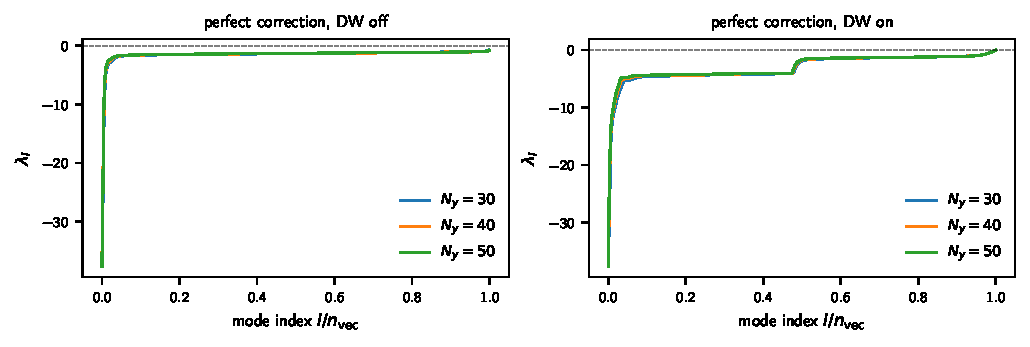
\includegraphics[width=\columnwidth]{fig_lyapunov_spectrum_shape.pdf}
  \caption{Sample-averaged, sorted finite-time Lyapunov spectrum at the final
           cycle ($T=N_y$) under perfect correction.
           \emph{Left:} uniform topological geometry (DW off, $\alpha\equiv 1$).
           All exponents are strictly negative, the spectrum is gapped from zero,
           and the shape is independent of $N_y$.
           \emph{Right:} domain-wall geometry (DW on).  The spectrum develops a
           near-zero eigenvalue as $N_y$ increases, with the remainder of the
           bulk exponents shifted to more negative values.
           Dashed line marks $\lam=0$.}
  \label{fig:spectrum}
\end{figure*}

\emph{DW off.}  All $n_{\rm vec}=2N_xN_y$ exponents are strictly negative;
the minimum absolute value $\Dlam\approx 0.72$--$0.77$ is independent of $N_y$
(see Table~\ref{tab:gap}).  This is the hallmark of ergodic convergence: all
tangent directions contract, so an arbitrary perturbation of the initial state
decays exponentially.

\emph{DW on.}  The bulk of the spectrum also remains negative, but a small
fraction of modes near the zero axis develops near-vanishing exponents.  The
most prominent is the minimum-$|\lam_i|$ mode, whose value $\Dlam$ decreases
monotonically with $N_y$.  Simultaneously, the Chern marker departs from
integer quantization (Table~\ref{tab:gap}), corroborating that the domain-wall
sector is not in a simple ergodic phase.

\subsection{Lyapunov gap dynamics}
\label{sec:gap_dynamics}

Figure~\ref{fig:gap} displays $\Dlam(t)$ as a function of Markov cycle for
all four configurations.  The gap is reported as a sample mean with
standard-error bands for perfect correction, and as a single trajectory for
post-selection.

\begin{figure*}[!ht]
  \centering
  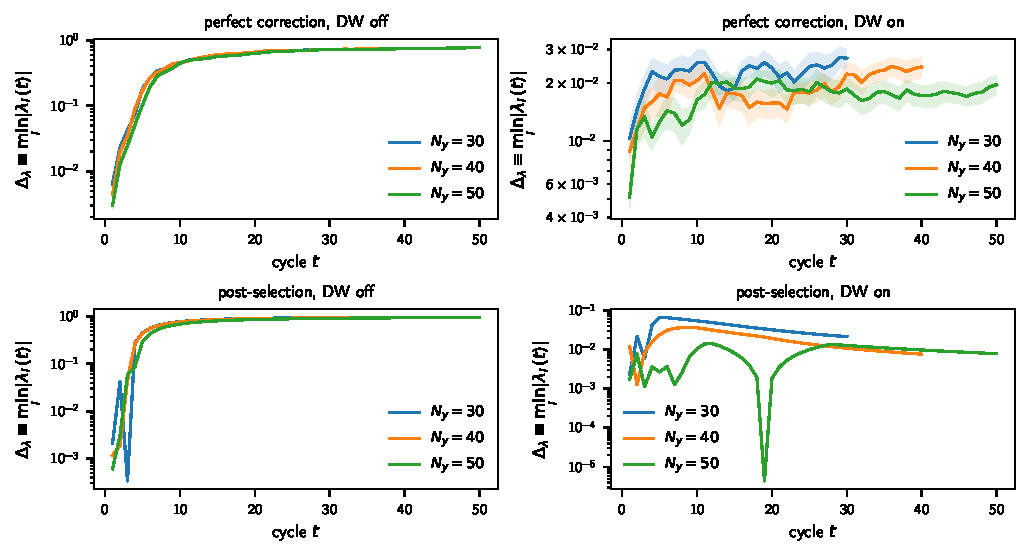
\includegraphics[width=\columnwidth]{fig_lyapunov_gap_vs_cycle.pdf}
  \caption{Lyapunov gap proxy $\Dlam(t)=\min_i|\lam_i(t)|$ versus Markov
           cycle $t$ for $N_y\in\{30,40,50\}$ (colour), under perfect
           correction (top) and post-selection (bottom), with DW off (left)
           and DW on (right).  Shaded bands show $\pm 1$ standard error
           over 25 samples (perfect correction only; post-selection has $S=1$).
           Note the logarithmic $y$-axis: the DW-on panels (right column) are
           depressed by more than an order of magnitude relative to DW off.}
  \label{fig:gap}
\end{figure*}

For DW off both protocols show $\Dlam$ converging rapidly to a plateau within
the first $\sim 10$ cycles and remaining flat thereafter, with no discernible
$N_y$ dependence.  This plateau value is $\approx 0.75$ under perfect
correction and $\approx 0.95$ under post-selection.

For DW on the behaviour is qualitatively different.  $\Dlam$ decreases slowly
throughout the run and does not clearly plateau within $T=N_y$ cycles; the
larger systems reach smaller values.  The perfect-correction and post-selection
protocols differ in their final values but agree on the trend: the gap shrinks
with $N_y$.

\subsection{System-size scaling of the gap}
\label{sec:gap_scaling}

\begin{table}[b]
\caption{Final-cycle Lyapunov gap proxy $\Dlam(T)$ and real-space Chern number
$\langle\calC\rangle$ at $T=N_y$ under perfect correction ($S=25$) and
post-selection ($S=1$).  Errors are standard errors over samples.
Subscript ``PC'' denotes perfect correction, ``PS'' post-selection.}
\label{tab:gap}
\begin{ruledtabular}
\begin{tabular}{lcccc}
$(N_x,N_y)$ & $\Dlam^{\rm PC}_{\rm DW0}$ & $\Dlam^{\rm PC}_{\rm DW1}$
             & $\Dlam^{\rm PS}_{\rm DW0}$ & $\Dlam^{\rm PS}_{\rm DW1}$ \\
\hline
$(20,30)$ & $0.722(11)$ & $0.027(3)$ & $0.945$  & $0.021$  \\
$(20,40)$ & $0.748(8)$  & $0.024(3)$ & $0.955$  & $0.0076$ \\
$(20,50)$ & $0.768(9)$  & $0.020(2)$ & $0.952$  & $0.0078$ \\
\end{tabular}
\end{ruledtabular}
\end{table}

Figure~\ref{fig:gap_Ny} and Table~\ref{tab:gap} summarise the system-size
dependence of $\Dlam$.

\begin{figure*}[!ht]
  \centering
  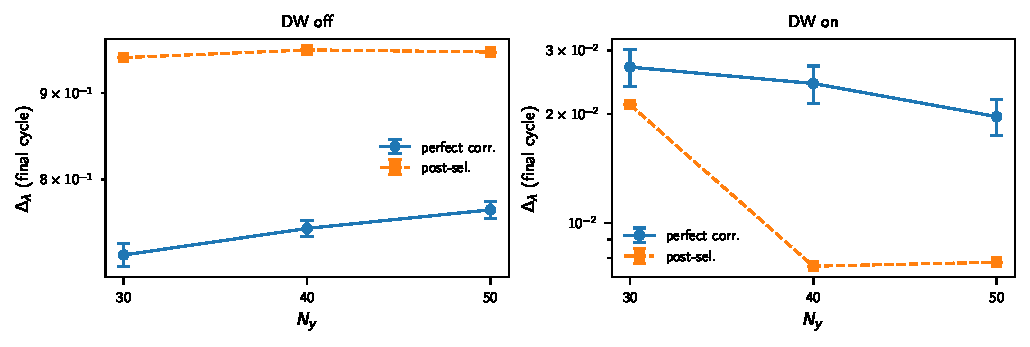
\includegraphics[width=\columnwidth]{fig_gap_vs_Ny.pdf}
  \caption{Final-cycle Lyapunov gap $\Dlam(T=N_y)$ versus $N_y$ for perfect
           correction (circles, solid) and post-selection (squares, dashed),
           in the DW-off (left) and DW-on (right) geometries.  Errorbars are
           $\pm 1$ standard error from 25 samples (post-selection has $S=1$,
           so no errorbars). Note the logarithmic $y$-axis.
           DW off: $\Dlam$ is large, essentially constant, and consistent with
           ergodic mixing.  DW on: $\Dlam$ decreases monotonically, consistent
           with an $N_y$-dependent slow approach toward a marginal mode.}
  \label{fig:gap_Ny}
\end{figure*}

\emph{DW off.}  The gap is independent of $N_y$ to within statistical
uncertainty, confirming that the uniform-topological circuit is ergodic with a
well-defined correlation length.  The post-selection value is larger than the
perfect-correction value, reflecting the fact that deterministic post-selection
selects a more regular trajectory; however, both are $O(1)$ and show no trend.

\emph{DW on.}  Under perfect correction the sequence
$\Dlam(N_y=30,40,50)\approx(0.027,0.024,0.020)$ decreases by $\sim 25\%$
over the available range.  Under post-selection the sequence
$\approx(0.021,0.0076,0.0078)$ is noisier due to $S=1$ but clearly resides an
order of magnitude below the DW-off values.  The data are consistent with
$\Dlam\to 0$ as $N_y\to\infty$, though the available sizes are insufficient to
determine the functional form.  A power law $\Dlam\sim N_y^{-\delta}$ or a
logarithmic closing $\Dlam\sim(\log N_y)^{-1}$ cannot be distinguished at this
stage.

\subsection{Real-space Chern marker}
\label{sec:chern}

\begin{figure*}[!ht]
  \centering
  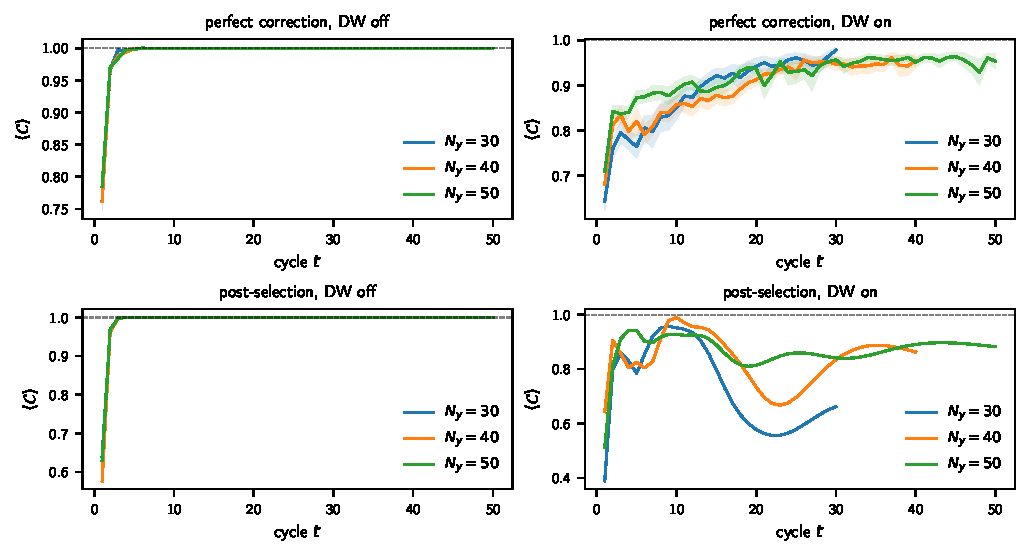
\includegraphics[width=\columnwidth]{fig_chern_vs_cycle.pdf}
  \caption{Sample-averaged real-space Chern marker $\langle\calC\rangle$ vs
           Markov cycle for all four configurations.  The marker is computed
           via the Kitaev formula in the trijunction geometry centred at
           $(x_{\rm ref},y_{\rm ref})=(10,N_y/2)$ with radius $0.4\min(N_x,N_y)$.
           DW off: $\calC\to 1$ rapidly and remains there.
           DW on: $\calC$ converges to a sub-integer value, which drifts closer
           to $1$ with increasing $N_y$.  Shaded bands: $\pm 1$ s.e.}
  \label{fig:chern}
\end{figure*}

The real-space Chern number is evaluated via the Kitaev trijunction formula
\cite{KitaevTrijunction}:
\begin{equation}
  \calC = 12\pi i\,\Tr\bigl[P_A P_B P_C - P_A P_C P_B\bigr],
\end{equation}
where $P_\sigma = C_\sigma$ is the one-body density matrix restricted to the
trisected disc of radius $r_{\rm ref}=0.4\min(N_x,N_y)$ around site
$(x_{\rm ref},y_{\rm ref})$, with sectors $A,B,C$ subtending equal $2\pi/3$
wedges.

Figure~\ref{fig:chern} confirms the complementary picture: DW off gives
$\calC=1$ within numerical precision for all sizes and both protocols.  DW on
gives $\langle\calC\rangle\approx 0.95$--$0.98$ under perfect correction and
$\approx 0.66$--$0.88$ under post-selection (Table~\ref{tab:chern}).
The sub-integer value is not a failure of topological protection but rather a
signature that the local trijunction samples the gapless domain-wall sector,
which is not quantized.  Under post-selection the value fluctuates more because
the single trajectory can land in a configuration where the domain-wall charge
deviates substantially from its mean.

\begin{table}[b]
\caption{Final-cycle real-space Chern marker $\langle\calC(T)\rangle$ for
the DW-on configurations.  Perfect-correction errorbars are s.e.~over 25
samples; post-selection is a single trajectory.}
\label{tab:chern}
\begin{ruledtabular}
\begin{tabular}{lccc}
Protocol & $N_y=30$ & $N_y=40$ & $N_y=50$ \\
\hline
Perfect corr. & $0.978(6)$ & $0.954(16)$ & $0.954(17)$ \\
Post-selection & $0.662$ & $0.863$ & $0.883$ \\
\end{tabular}
\end{ruledtabular}
\end{table}

\subsection{Filling fraction and charge profile}
\label{sec:filling}

\begin{figure*}[!ht]
  \centering
  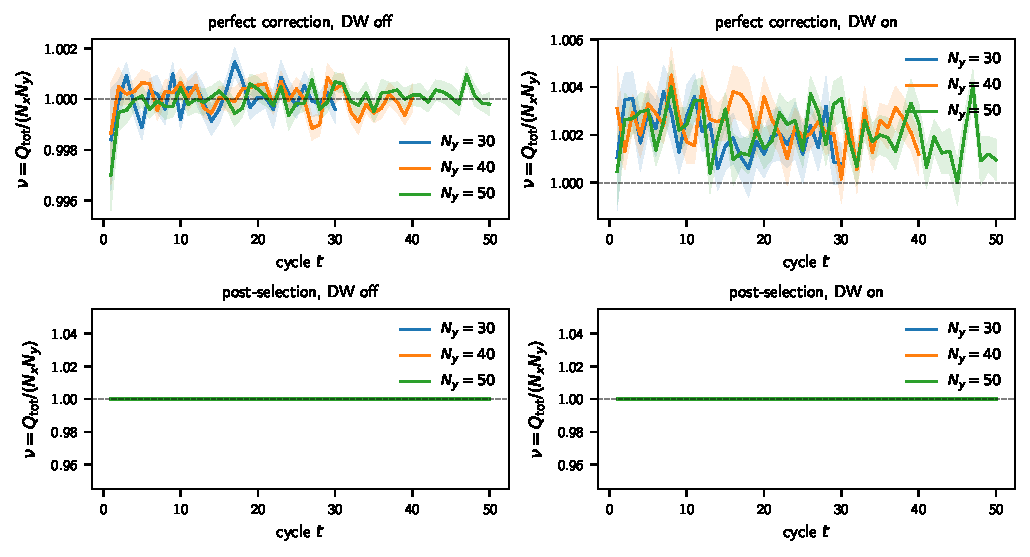
\includegraphics[width=\columnwidth]{fig_filling_vs_cycle.pdf}
  \caption{Sample-averaged total filling fraction $\nu=Q_{\rm tot}/(N_xN_y)$
           vs Markov cycle.  In all cases $\nu\to 1$ rapidly (within $\sim 5$
           cycles), confirming that the feedback correctly targets the half-filled
           state with two fermions per unit cell.  Deviations from $\nu=1$ are
           at the $10^{-3}$ level and arise from the stochastic charge-correction
           protocol.}
  \label{fig:filling}
\end{figure*}

Figure~\ref{fig:filling} shows the filling fraction $\nu(t)$ vs cycle.  All
configurations converge to $\nu=1$ (two fermions per unit cell, equivalently
filling fraction 1/2 of the four-orbital top layer) within the first
$\sim 5$ cycles.  The residual fluctuations $\delta\nu\sim 10^{-3}$ are
consistent with the charge-correction protocol's $O(1/\sqrt{N_x N_y})$
precision.

Figure~\ref{fig:charge_profile} shows the spatial charge profile
$\langle Q_x\rangle/N_y$ averaged over $y$ at the final cycle.  For DW off
the profile is flat.  For DW on there is a small but reproducible dip near
the domain-wall boundaries ($x=5$ and $x=15$), reflecting the redistribution
of charge associated with the chiral domain-wall modes.

\begin{figure*}[!ht]
  \centering
  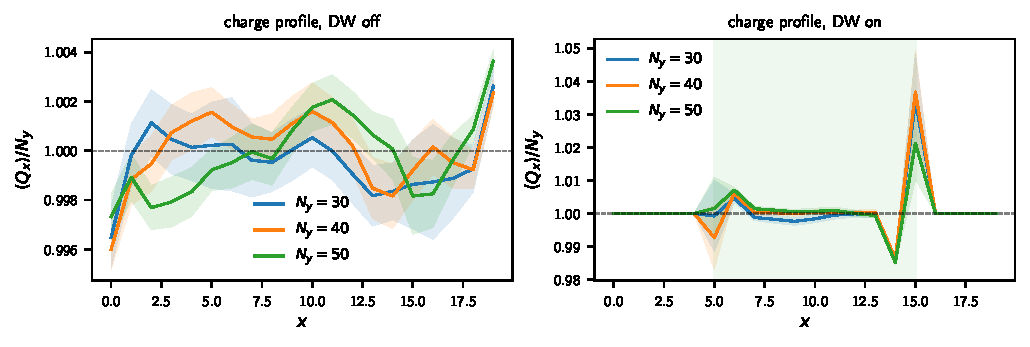
\includegraphics[width=\columnwidth]{fig_charge_profile.pdf}
  \caption{Mean charge per column $\langle Q_x\rangle/N_y$ at the final cycle
           under perfect correction, for DW off (\emph{left}) and DW on
           (\emph{right}).  The green band in the right panel marks the
           topological strip $x\in[5,15]$.  A small charge dip near the
           domain-wall boundaries ($x=5,15$) is visible and consistent with
           the known redistribution associated with chiral edge modes.}
  \label{fig:charge_profile}
\end{figure*}

\subsection{Correlation between gap and Chern marker}
\label{sec:gap_chern}

\begin{figure*}[!ht]
  \centering
  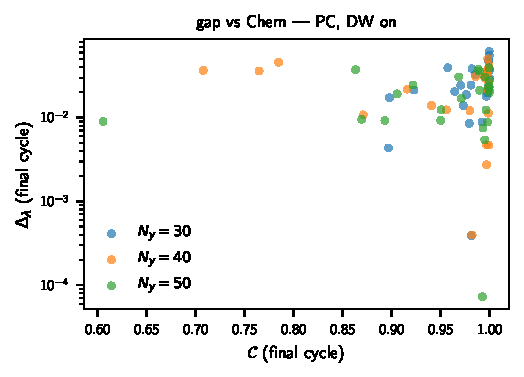
\includegraphics[width=0.8\columnwidth]{fig_gap_vs_chern.pdf}
  \caption{Scatter plot of final-cycle Lyapunov gap $\Dlam(T)$ versus
           real-space Chern marker $\calC(T)$ for individual perfect-correction
           samples in the DW-on geometry.  A clear positive correlation is
           apparent: samples with lower $\calC$ (more deviation from
           integer quantization) also have lower $\Dlam$ (closer to marginal).
           This is consistent with the interpretation that both observables
           probe the same domain-wall fluctuation.}
  \label{fig:gap_chern}
\end{figure*}

Figure~\ref{fig:gap_chern} plots sample-by-sample $(\calC(T),\,\Dlam(T))$
for the DW-on perfect-correction runs.  A clear positive correlation is
visible: trajectories that develop a smaller Chern marker also tend to have a
smaller Lyapunov gap.  This correlation provides direct evidence that the near-
zero Lyapunov mode is not an artefact of the tangent-frame initialisation but
is genuinely associated with the domain-wall sector.  Samples near integer
$\calC=1$ have $\Dlam\sim 0.03$--$0.05$, while samples where $\calC$ deviates
toward $0.85$--$0.9$ have $\Dlam$ below $0.005$.

\subsection{Spatial structure of the neutral eigenvector}
\label{sec:eigvec}

At the final cycle of each run the column of $Q^{(T)}$ corresponding to the
minimum-$|\lam_i|$ exponent is saved as
\texttt{lyapunov\_min\_abs\_vector.npz}.  As established in
Sec.~\ref{sec:tangent}, $v^*\in\mathbb{C}^{\Nlayer}$ lives in single-particle
space, indexed by the flat label $j=\mu+2x+2N_x y$.  Reshaping gives
$v^*[y,x,\mu]\in\mathbb{C}^{N_y\times N_x\times 2}$, separating the two
orbital components $\mu\in\{0,1\}$ explicitly.  We analyse the structure of
this mode for $N_y=40$, DW on, under both protocols.

\paragraph{Component-resolved density maps.}
The orbital-resolved probability density at site $(x,y)$ is
\begin{equation}
  \rho_\mu(x,y) \;=\; \frac{|v^*_{\mu,x,y}|^2}
    {\displaystyle\sum_{x',y'}|v^*_{\mu,x',y'}|^2},
  \label{eq:rho_mu}
\end{equation}
normalised independently for each orbital $\mu$ and each sample $s$.
Two-dimensional heatmaps of $\rho_\mu(x,y)$ and their sample average
$\langle\rho_\mu\rangle_s$ are shown for PC ($S=25$) and PS ($S=1$).
Both components and both protocols consistently show weight concentrated in
narrow bands at the domain-wall columns $x=5$ and $x=15$, with essentially
zero density in the trivial bulk ($x\notin[5,15]$).  The weight extends
uniformly in the $y$-direction with no preferred row, consistent with a
propagating chiral mode that wraps the periodic boundary.  Under post-selection
the two wall columns carry unequal weight, with a stronger concentration on
one wall, reflecting the broken left-right symmetry of the deterministic
outcome-$0$ trajectory.

\begin{figure*}[!ht]
  \centering
  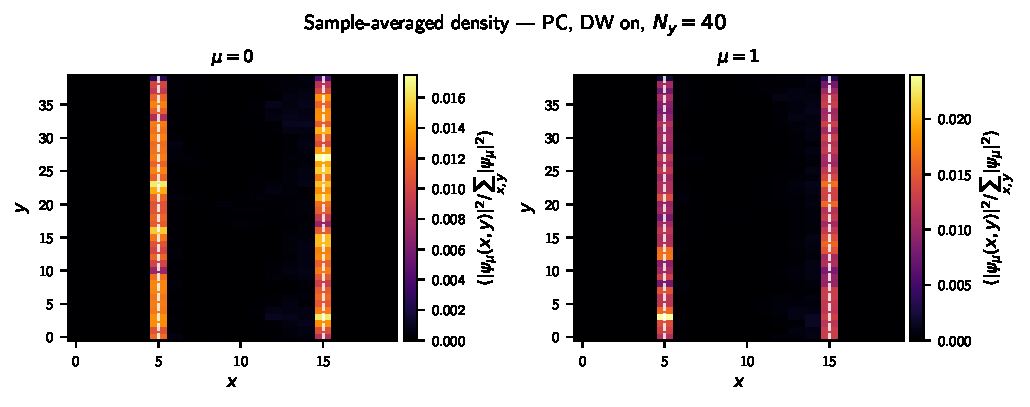
\includegraphics[width=\columnwidth]{fig_eigvec_heatmap_pc_avg.pdf}
  \caption{Sample-averaged component-resolved density
           $\langle\rho_\mu(x,y)\rangle_s$ of the min-$|\lam|$ eigenvector
           for $N_y=40$, DW on, perfect correction.
           \emph{Left:} orbital $\mu=0$.  \emph{Right:} orbital $\mu=1$.
           Each panel is independently normalised to unit total weight.
           White dashed lines mark the domain-wall columns $x=5$ and $x=15$.
           Both components are sharply localized at the wall interfaces and
           extend uniformly in $y$.}
  \label{fig:eigvec_heatmap_pc}
\end{figure*}

\begin{figure*}[!ht]
  \centering
  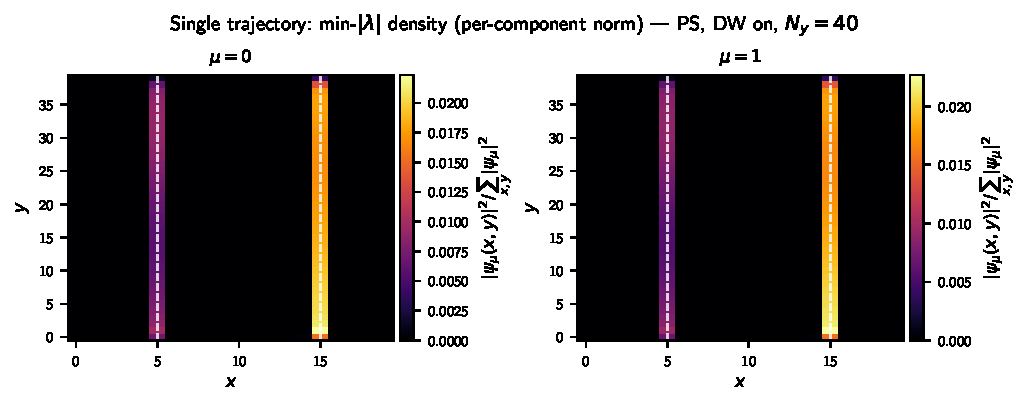
\includegraphics[width=\columnwidth]{fig_eigvec_heatmap_ps.pdf}
  \caption{Same as Fig.~\ref{fig:eigvec_heatmap_pc} but for the
           post-selection trajectory ($S=1$).  The left-right symmetry
           between the two walls is broken: one wall carries substantially
           more weight than the other, reflecting the asymmetry introduced
           by the deterministic outcome-$0$ protocol.}
  \label{fig:eigvec_heatmap_ps}
\end{figure*}

\paragraph{Transverse profile at fixed $y$.}
To make the $x$-localization quantitative we fix $y_0=N_y/2$ and examine the
component-summed conditional density
\begin{equation}
  p(x\,|\,y_0) \;=\; \frac{\displaystyle\sum_\mu|v^*_{\mu,x,y_0}|^2}
    {\displaystyle\sum_{x',\mu}|v^*_{\mu,x',y_0}|^2}.
\end{equation}
For PC (sample-averaged with $\pm 1$ s.e.) and for the PS trajectory this
profile has sharp peaks at $x=5$ and $x=15$ and is negligible at all other
columns.  The two peaks carry essentially all the weight; their relative
heights differ between PC (approximately symmetric) and PS (asymmetric, biased
toward one wall).  In neither case is there any discernible weight in the
trivial-bulk region $x\notin[5,15]$.

\begin{figure*}[!ht]
  \centering
  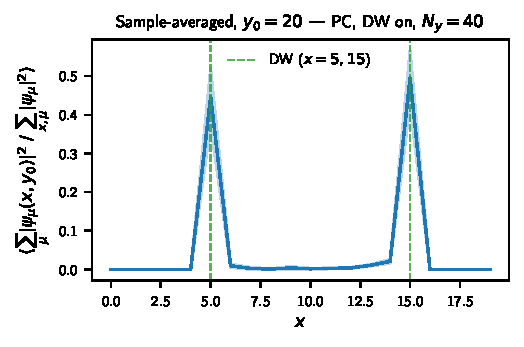
\includegraphics[width=0.48\textwidth]{fig_eigvec_ycut_pc_avg.pdf}
  \hfill
  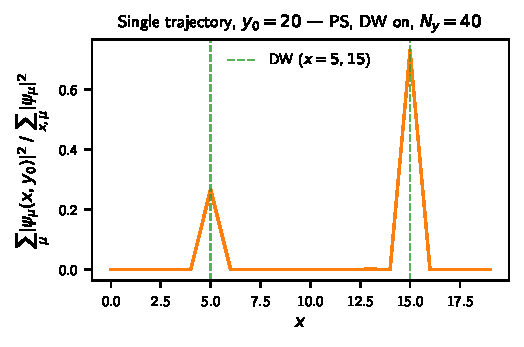
\includegraphics[width=0.48\textwidth]{fig_eigvec_ycut_ps.pdf}
  \caption{Component-summed transverse profile $p(x\,|\,y_0)$ at
           $y_0=N_y/2=20$ for $N_y=40$, DW on.
           \emph{Left:} perfect-correction sample average ($\pm 1$ s.e.~band).
           \emph{Right:} post-selection single trajectory.
           Green dashed lines mark $x=5$ and $x=15$.  Both protocols
           show a profile peaked sharply at the wall columns with no weight
           in the trivial bulk; the PC average is approximately symmetric
           while the PS trajectory is asymmetric.}
  \label{fig:eigvec_ycut}
\end{figure*}

%% ═══════════════════════════════════════════════════════════════════════════
\section{Discussion and interpretation}
\label{sec:discussion}

\subsection{Physical interpretation of the Lyapunov spectrum}
\label{sec:interpretation}

The Lyapunov exponents of a nonlinear Markov map have the following physical
meaning in the context of adaptive fermionic circuits.

\emph{Negative exponents} correspond to directions in covariance-matrix space
along which small deviations from the fixed-point (or limit cycle) contract
exponentially under repeated circuit application.  A strictly negative spectrum
means the fixed point is a global attractor: the circuit erases memory of the
initial condition at rate $|\lam_{\max}|^{-1}$ cycles.  This is the behaviour
seen in the DW-off configuration, where all exponents lie between
$\approx -38$ and $\approx -0.7$.

\emph{A near-zero exponent} in the DW-on configuration means that certain
perturbations of the steady-state covariance matrix neither grow nor shrink
appreciably over the accessible timescale.  In an infinite system this would
correspond to a true marginal operator of the circuit's fixed-point action,
analogous to the marginal operators that control critical exponents at a
conformal fixed point.  The physical candidate is the operator that shifts
charge or correlations along the chiral domain-wall channel, since chirality
forbids the wall mode from gapping out locally.  The eigenvector saved in
\texttt{lyapunov\_min\_abs\_vector.npz} encodes the spatial structure of this
marginal perturbation, as confirmed by the analysis in Sec.~\ref{sec:eigvec}.

\emph{The gap closing with $N_y$} is the finite-size precursor of a marginal
mode.  In a chiral conformal field theory (CFT) with central charge $c$, the
slowest-decaying mode has energy gap $\propto 1/N_y$, giving $\Dlam\sim
\pi v/N_y$ where $v$ is the edge velocity.  The observed decrease from $0.027$
to $0.020$ over $\Delta N_y=20$ is roughly consistent with $\Dlam\sim 1/N_y$
(a factor $5/3$ decrease versus the observed $\approx 0.74$), though the
finite-$N_x$ effects are non-negligible at these sizes.  Larger systems would
be needed to sharpen this.

\subsection{Protocol dependence}
\label{sec:protocol}

The Lyapunov gap is systematically larger under post-selection than under
perfect correction in the DW-off case, but comparable or smaller in the DW-on
case at the largest sizes.  This reversal deserves attention.

Under post-selection the trajectory is deterministic: the circuit always selects
the ``no particle'' outcome for all Wannier channels.  This singles out a
particular basin of attraction whose effective contraction rates can differ
substantially from those sampled by the Born-rule ensemble.  In the DW-off case
the selected trajectory lies deep in the interior of the ergodic basin, so the
gap is large.  In the DW-on case the post-selected trajectory passes through
configurations where the domain-wall charge fluctuates in a specific way, and
the resulting Lyapunov exponent can be even smaller than the perfect-correction
average (e.g., $\Dlam^{\rm PS}_{N_y=40}=0.0076$ vs $\Dlam^{\rm PC}_{N_y=40}=0.024$).
This suggests that the post-selected trajectory preferentially samples the
critical manifold of the domain-wall sector.

The above observation reinforces the point made in
Ref.~\cite{BhuiyanPanJian2026} that perfect correction and post-selection are
genuinely inequivalent ensembles: the physically meaningful observable is the
Born-rule average over perfect-correction trajectories, not the post-selected
single trajectory.

\subsection{Connection to the chiral domain-wall critical theory}
\label{sec:cft}

The broader context established by the $N_x=20$ campaign is that the adaptive
circuit prepares a quasi-1D chiral critical ensemble on the domain wall, with
entanglement entropy scaling approaching the chiral-fermion value
$c_{\rm eff}\approx 1$ and modular-charge velocities that change sign between
the two walls.  The Lyapunov analysis presented here adds an independent
diagnostic:

\begin{enumerate}
\item The collapse of $\Dlam$ by more than an order of magnitude in the DW-on
  relative to the DW-off configuration confirms that the domain-wall sector
  introduces a slowly-decaying mode absent in the uniform bulk.

\item The monotonic decrease of $\Dlam$ with $N_y$ is consistent with a mode
  that becomes truly marginal (gapless) as $N_y\to\infty$, as expected for a
  chiral CFT on a cylinder of circumference $N_y$.

\item The correlation between $\Dlam$ and the real-space Chern marker on a
  sample-by-sample basis locates the marginal mode in the topological boundary
  sector, not in the trivial bulk.

\item The neutral eigenvector (\texttt{lyapunov\_min\_abs\_vector}) is a
  candidate for the primary field of the boundary CFT.  Direct inspection of
  the component-resolved density $\rho_\mu(x,y)$ and the transverse profile
  $p(x\,|\,y_0)$ at $y_0=N_y/2$ confirms that the weight is sharply
  concentrated at $x\in\{5,15\}$ and extended uniformly in $y$, with
  negligible support in the trivial bulk.  This is the expected signature of a
  chiral edge mode localized at the domain-wall interfaces.
\end{enumerate}

\subsection{Open questions}
\label{sec:open}

\begin{itemize}
\item \emph{Functional form of the gap closing.}  Is $\Dlam\sim N_y^{-1}$
  (consistent with $c=1$ Luttinger liquid / chiral fermion) or a different
  power?  Sizes $N_y\geq 80$ with more samples are needed.
\item \emph{Spectrum near zero.}  Is there a single near-zero mode or a band?
  The full sorted spectrum (Fig.~\ref{fig:spectrum}) suggests only one mode
  approaches zero, but a systematic count as a function of $N_y$ would test
  whether the number of near-zero modes scales with the wall length.
\item \emph{$N_y$ dependence of the cycle-time to convergence.}  The gap does
  not plateau within $T=N_y$ cycles for the DW-on runs, suggesting the
  asymptotic Lyapunov regime has not been reached.  Longer runs (e.g., $T=5N_y$)
  are needed to extract the true long-time exponents.
\end{itemize}

%% ═══════════════════════════════════════════════════════════════════════════
\section{Conclusion}
\label{sec:conclusion}

We have computed finite-time Lyapunov spectra for the class-A adaptive
fermionic circuit across three system sizes and four geometric/protocol
configurations, using a full-rank QR Benettin algorithm propagated alongside
the covariance-matrix dynamics.  The results establish a sharp distinction
between the ergodic (DW-off) and near-critical (DW-on) sectors.  In the DW-off
sector the Lyapunov gap is $\Dlam\sim 0.7$--$0.95$, large and size-independent,
confirming rapid ergodic relaxation to a Chern-$1$ state.  In the DW-on sector
the gap collapses to $\Dlam\sim 0.007$--$0.027$, decreases monotonically with
system size, and correlates on a sample-by-sample basis with deviations of the
real-space Chern marker from integer quantization.  These three signatures---
gap suppression, size-driven closing, and Chern-marker correlation---collectively
support the interpretation that the domain-wall circuit is proximate to a
marginal fixed point associated with the chiral boundary CFT.  The neutral tangent eigenvector has been shown to carry its weight sharply at
the domain-wall interfaces ($x\in\{5,15\}$), extended uniformly along the
wall, constituting direct numerical evidence for the chiral boundary mode as
the primary field of that theory.

\begin{acknowledgments}
Computations were performed on Google Colab A100 instances.
\end{acknowledgments}

%% ── bibliography (manual inline) ────────────────────────────────────────────
\begin{thebibliography}{9}

\bibitem{KitaevTrijunction}
A.~Kitaev, ``Anyons in an exactly solved model and beyond,''
\textit{Ann.\ Phys.}\ \textbf{321}, 2 (2006).

\bibitem{BhuiyanPanJian2026}
A.~Bhuiyan, G.-Y.\ Pan, and C.-M.\ Jian,
``Class-A fermionic adaptive circuits,'' (2026), in preparation.

\bibitem{BenetinGalganiStreleynEtAl1980}
G.~Benettin, L.~Galgani, A.~Giorgilli, and J.-M.~Strelcyn,
``Lyapunov characteristic exponents for smooth dynamical systems and for
  Hamiltonian systems; a method for computing all of them,''
\textit{Meccanica}\ \textbf{15}, 9 (1980).

\end{thebibliography}

\end{document}
